\section{Graphical Frontends}
Es gibt eine große Auswahl von graphischen Benutzeroberflächen um auf Subversion-Repositorys zuzugreifen. Sie vereinfachen den Umgang mit SVN enorm, da komplett auf die Kommandozeilen Eingabe verzichtet wird.\\
Drei verschiedene Arten von GUIs werden wir hier nun kurz  vorstellen:
\subsection{SmartSVN}
SmartSVN ist ein eigenständies Programm, das auf den Betriebssystemen Linux, UNIX, Mac OS X, Windows lauffähig ist. Im Internet ist eine gratis Demoversion für 30Tage auffindbar, wenn man allerdings die Vollversion benutzen möchte, muss man dafür zahlen.\\
Neben dem Standalone-Client integriert sich SmartSVN unter Windows zusätzlich auch noch in den Explorer (Abbildung \ref{fig:smart1}). Das Menü bietet eine übersichtliche Dateiverwaltung (Abbildung \ref{fig:smart2}) und optisch gut aufbereitete Vergleiche der Versionen an (Abbildung \ref{fig:smart3}).
Neben dem HTTP-Protokoll, werden auch noch HTTPS, SVN, und SVN+SSH unterstützt\footnote{Quelle: \url{http://www.syntevo.com/smartsvn}}.
\begin{figure}[!htb]
        \centering
        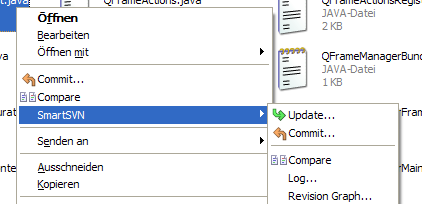
\includegraphics[width=.8\textwidth]{1_smartsvn1.png}
        \caption{SmartSVN: Shell-Integration}
        \label{fig:smart1}
\end{figure}
\begin{figure}[!htb]
        \centering
        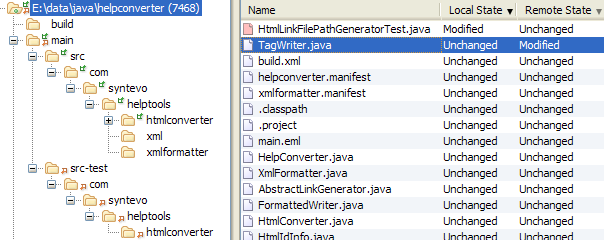
\includegraphics[width=.9\textwidth]{2_smartsvn2.png}
        \caption{SmartSVN: Dateiverwaltung}
        \label{fig:smart2}
\end{figure}
\begin{figure}[!htb]
        \centering
        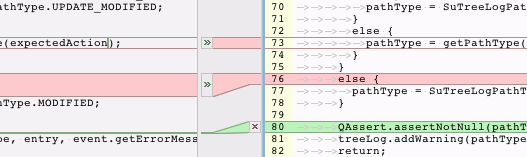
\includegraphics[width=.9\textwidth]{3_smartsvn3.png}
        \caption{SmartSVN: Unterschiedskontrolle}
        \label{fig:smart3}
\end{figure}
\subsection{Tortoise SVN}
Tortoise hingegen ist ein kostenloser Windows-Client der unter der GNU GPL Lizenz steht. Es integriert sich ebenfalls in den Windows-Explorer und ist deshalb ebenfalls außerhalb und unabhängig von einer IDE verwendbar. Im Gegensatz zu SmartSVN ist TortoiseSVN aber kein standalone-Client, sondern bietet nur die reine Shell-Extension (Abbildung \ref{fig:tortoise1}).
Zur Zeit ist die Software in 34 Sprachen verfügbar.
Die unterstützten Protokolle sind: http, https, svn, svn+ssh, file und svn+xxx\footnote{Quelle: \url{http://tortoisesvn.tigris.org/}, \url{http://de.wikipedia.org/wiki/TortoiseSVN}}.
\begin{figure}[!htb]
	\centering
	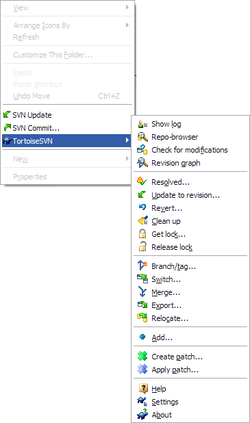
\includegraphics[width=.45\textwidth]{4_turtoise1.png}
	\caption{Bildbeschreibung}
	\label{fig:tortoise1}
\end{figure}  
\subsection{Subclipse SVN}
Subclipse ist die dritte GUI Variante, die nun hier vorgestellt wird. Anders als die beiden vorhergegangenen Programme integriert sich Subclipse direkt in die Entwicklungsumgebung Eclipse.\\
Das Eclipse-Plugin steht unter der EPL-Lizenz und ist unter den Betriebssystemen Linux, Mac OS X und Windows lauffähig. Subclipse unterstützt die folgenden Protokolle: http, https, svn, svn+ssh und file. Neben dem Vorteil die Dateien direkt vom SVN Repository in die IDE zu laden, bietet Subclipse zusätzlich ansprechende Features wie z.B. die Generierung von Versionsgraphen.\footnote{Quelle: \url{http://subclipse.tigris.org/}}
\begin{figure}[!htb]
        \centering
        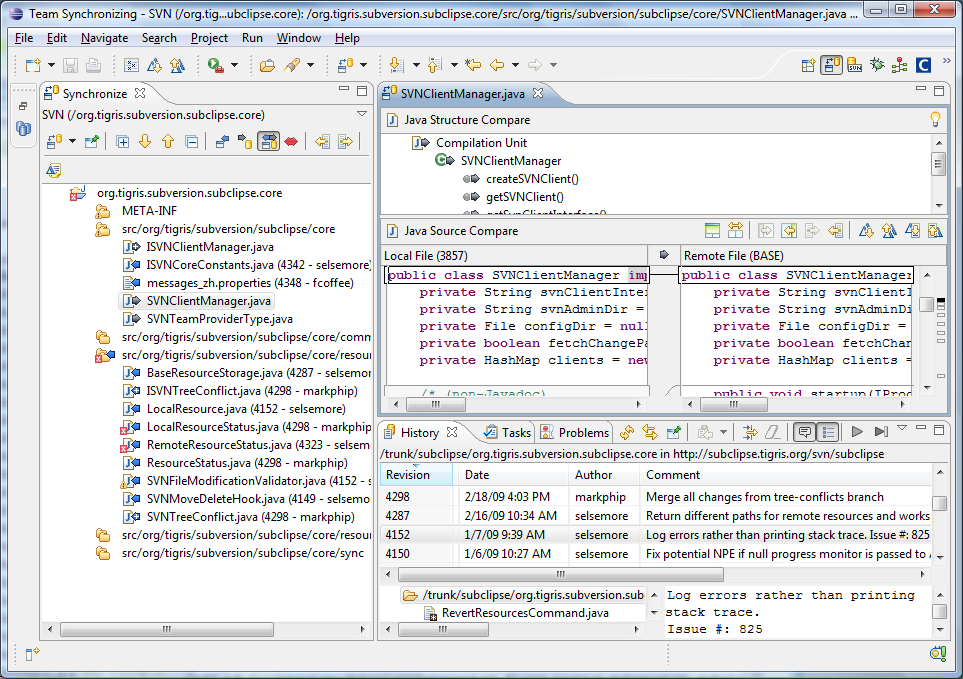
\includegraphics[width=.8\textwidth]{5_subclipse1.png}
        \caption{Subclipse: Eclipse Synchronize View}
        \label{fig:subclipse1}
\end{figure}
